\chapter{Question 2}
\label{avoiding-uri-aliases} 

\textbf {Choose a query term (e.g., ``shadow'') that is not a stop word (see week 5 slides) and not HTML markup from step 1 (e.g., ``http'') that matches at least 10 documents (hint: use ``grep'' on the processed files).  If the term is present in more than 10 documents, choose any 10 from your list.  (If you do not end up with a list of 10 URIs, you've done something wrong).}
\textbf {As per the example in the week 5 slides, compute TFIDF values for the term in each of the 10 documents and create a table with the TF, IDF, and TFIDF values, as well as the corresponding URIs.  The URIs will be ranked in decreasing order by TFIDF values.  For example:
Table 1. 10 Hits for the term ``shadow'', ranked by TFIDF.}

\textbf{\\
TFIDF \qquad TF	  \qquad IDF	\qquad \qquad URI\\
----- \qquad \qquad --	  \qquad ---\qquad \qquad \qquad ---\\
0.150 \qquad 0.014\qquad 10.680\qquad http://foo.com/\\
0.044 \qquad 0.008\qquad 5.510\qquad http://bar.com/\\
You can use Google or Bing for the DF estimation.  To count the number of words in the processed document (i.e., the denominator for TF), you can use ``wc'':\\
wc -w www.cnn.com.processed\\
2370 www.cnn.com.processed}\\
\textbf{It won't be completely accurate, but it will be probably be consistently inaccurate across all files.  You can use more  accurate methods if you'd like.\\
Don't forget the log base 2 for IDF, and mind your significant digits!}

Following are the steps that I have taken to solve this problem:
\begin{itemize}
\item I made use of the processed data generated in question 1 and selected a query term.\\
\item Using the following cURL command, I searched for the query term in processed files to find the frequency of the term in each URI.\\
cat ./processedData/ $<$filename$>$ | grep -i -c $<$queryTerm$>$
\item First I looked for the word `America' in all the processed files. I got more than 10 URIs, But the number of times the query term appeared in each URI was not satisfactory.The screenshot of the output with filename and number of times the word `America' appeared in each file is in Figure \ref{fig:q2fig1}.
\item Then I changed my query term to `food' which gave a better frequency. The screenshot for this output is in Figure \ref{fig:q2fig2}
\item I also counted the total number of words in each processed file using the command:\\
cat ./processedData/ $<$filename$>$ | wc -w. 
\item Then I stored the output in a JSON structure with file name, total number of words in the document and frequency of the query term in the document. This code is listed in Listing \ref{lst:q2code1} and screenshot of this JSON structure is in Figure \ref{fig:q2fig3}.
\item When I searched for the term `food' I received about 338 URIs but I selected 10 URIs among them based on the versatility of the frequency of the term in each document.
\item The selected 10 URIs are as follows:\\
{\url{http://www.chilipeppermadness.com/}}\\
{\url{http://tcbmag.com/Innovations/January-2016/Why-Chipotle-Is-Closing-Its-Stores-Over-The-Lunch?utm_content=27945314&utm_medium=social&utm_source=twitter}}\\
{\url{http://www.CafeRio.com }}\\
{\url{http://www.yelp.com/biz/chipotle-mexican-grill-gainesville-4?utm_campaign=CheckIn&utm_medium=twitter&utm_source=ashare}}\\
{\url{http://www.nydailynews.com/life-style/eats/chipotle-lettuce-shortage-plagues-new-york-article-1.2520586}}\\
{\url{http://fieryfork.com/video-chipotle-profit-heats-up-as-it-draws-more-diners/}}\\
{\url{http://www.eater.com/2016/2/5/10922434/chipotle-e-coli-beef-australia?utm_campaign=national&utm_medium=social&utm_source=twitter}}\\
{\url{http://www.havingfunsaving.com/2016/01/chipotle-cheese-dip-recipe.html}}\\
{\url{http://www.ooyuz.com/geturl?aid=10248937}}\\
{\url{http://smartmarkradio.com/conspiracy-theory-news/this-chipotle-conspiracy-theory-is-the-craziest-thing-weve-read-all-day-grist/}}
\item To calculate IDF for these URIs, I got the total number of documents in corpus which was 47 billion and documents with the term `food' which was about 3.52 billion.
\item Then I calculated the values of TF, IDF, TFIDF. The code is listed in Listing \ref{lst:q2code2}
\item These values are summarized in the Table \ref{Table:q2table1}.
\end{itemize}

\newpage
\begin{table}

\caption{Table with calculated TFIDF , TF , IDF and URI}
\label{Table:q2table1}
\begin{center}
\begin{tabular}{ c | c | c | c | p{10cm} }
\hline
Rank & TFIDF & TF & IDF & URI \\ \hline

1 & 0.075 & 0.02 & 3.739 & http://fieryfork.com/video-chipotle-profit-heats-up-as-it-draws-more-diners/ \\ \hline
2 & 0.045 & 0.012 & 3.739 & http://www.chilipeppermadness.com/ \\ \hline
3 & 0.026 & 0.007 & 3.739 & http://www.nydailynews.com/life-style/eats/chipotle-lettuce-shortage-plagues-new-york-article-1.2520586 \\ \hline
4 & 0.022 & 0.006 & 3.739 & http://tcbmag.com/Innovations/January-2016/Why-Chipotle-Is-Closing-Its-Stores-Over-The-Lunch?... \\ \hline
5 & 0.019 & 0.005 & 3.739 & http://www.CafeRio.com \\ \hline
6 & 0.019 & 0.005 & 3.739 & http://www.eater.com/2016/2/5/10922434/chipotle-e-coli-beef-australia?utm\textunderscore ... \\ \hline
7 & 0.019 & 0.005 & 3.739 & http://www.ooyuz.com/geturl?aid=10248937 \\ \hline
8 & 0.011 & 0.003 & 3.739 & http://www.yelp.com/biz/chipotle-mexican-grill-gainesville-4?utm\textunderscore campaign=... \\ \hline
9 & 0.011 & 0.003 & 3.739 & http://smartmarkradio.com/conspiracy-theory-news/this-chipotle-conspiracy-theory-is-the-craziest... \\ \hline
10 & 0.007 & 0.002 & 3.739 & http://www.havingfunsaving.com/2016/01/chipotle-cheese-dip-recipe.html \\ \hline
\hline

\end{tabular}
\end{center}
\end{table} 


\newpage
\begin{figure}[h!]
\begin{center}
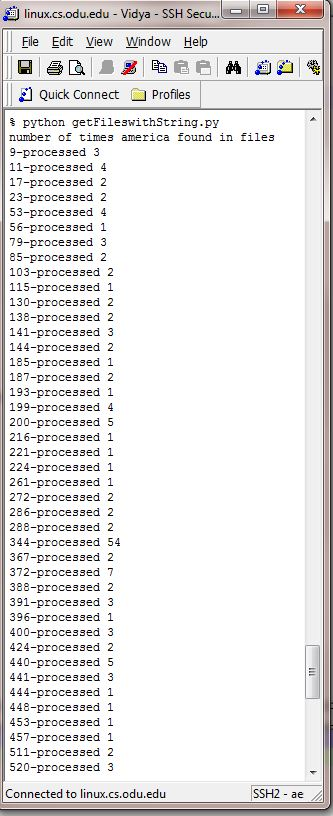
\includegraphics[scale=0.55, keepaspectratio=true]{figures/america.JPG}
\caption{Number of times ``America'' appeared in processed files}
\label{fig:q2fig1}
\end{center}
\end{figure}

\newpage
\begin{figure}[h!]
\begin{center}
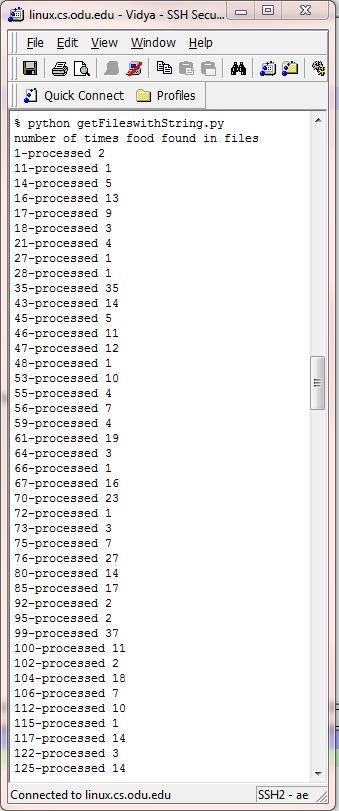
\includegraphics[scale=0.55, keepaspectratio=true]{figures/food.JPG}
\caption{Number of times ``food'' appeared in processed files}
\label{fig:q2fig2}
\end{center}
\end{figure}

\newpage
\begin{figure}[h!]
\begin{center}
\hspace*{-1.5in}
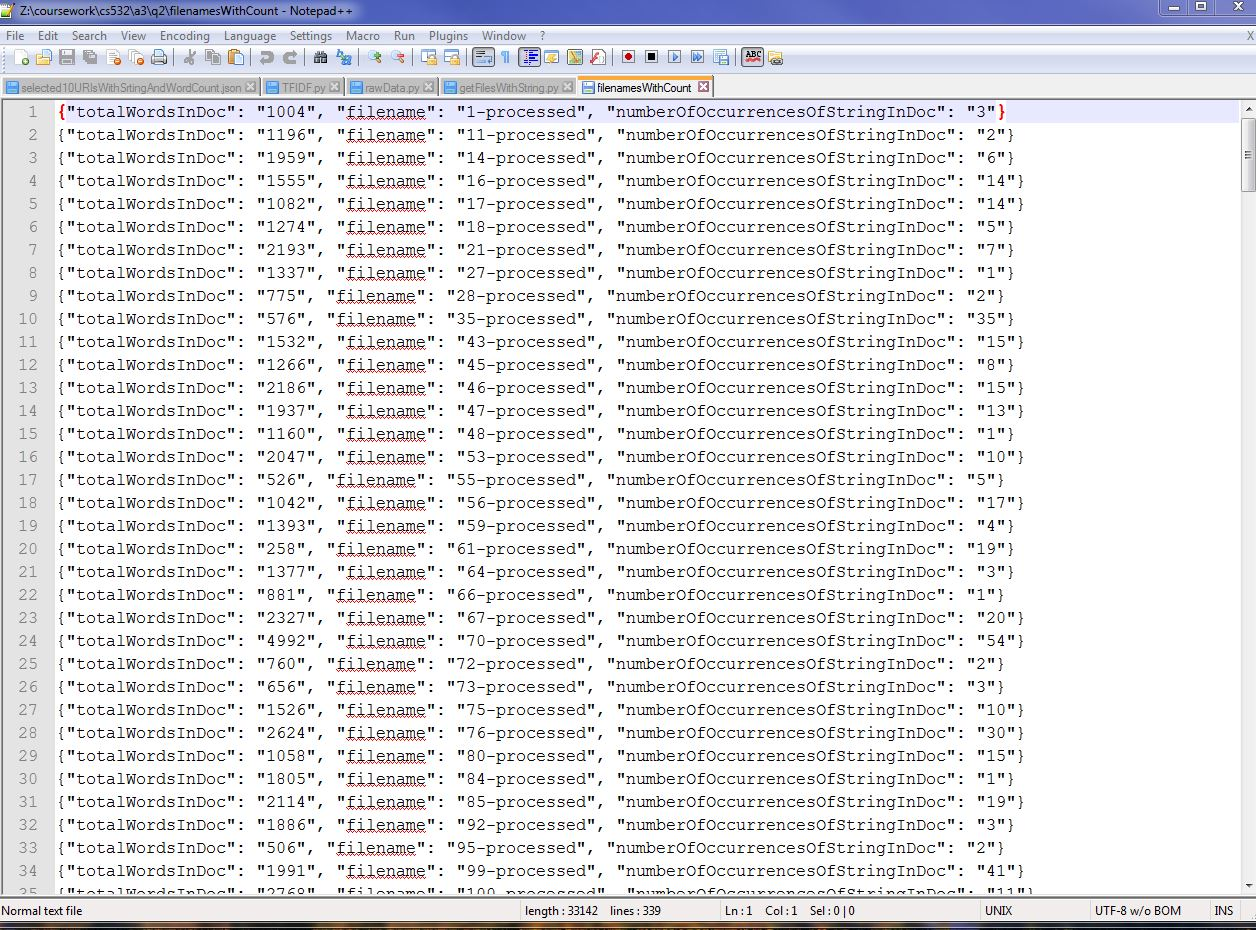
\includegraphics[scale=0.55, keepaspectratio=true]{figures/JSONstructure.JPG}
\caption{JSON structure with file name, total number of words in processed file and number of times the query term occurred in the file}
\label{fig:q2fig3}
\end{center}
\end{figure}


\newpage
\textbf{Code Listing}
\lstinputlisting[language=Python,caption=``Python code for searching a query term and counting the number of times the term appears in each processed file. Also counted the total number of words in each processed file and have written the output in a JSON structure.'',frame=single,label=lst:q2code1,breaklines=true,captionpos=b,numbers=left,showspaces=false,showstringspaces=false,basicstyle=\footnotesize]{src/getFilesWithString.py}

\newpage
\textbf{Code Listing}
\lstinputlisting[language=Python,caption=``Python code for calculating TF{,} IDF and TFIDF for 10 selected URIs'',frame=single,label=lst:q2code2,breaklines=true,captionpos=b,numbers=left,showspaces=false,showstringspaces=false,basicstyle=\footnotesize]{src/TFIDF.py}


